\section{Introduction}
\label{sec:intro}

Human readers do not process a document page uniformly or strictly in layout order. Under a limited attention budget, they first focus on regions that carry the most information, such as text, formulas, tables, and structural boundaries, while assigning lower priority to blank margins, line spacing, paper texture, and background areas. Importantly, these low-priority cues are not discarded entirely; they are compressed into coarser contextual representations. This ``rank first, compress later'' behavior allows humans to read complex pages efficiently with limited cognitive resources.

End-to-end document VLMs simplify traditional OCR pipelines by directly mapping a full page image to structured OCR outputs, avoiding the coupling among detection, recognition, and reconstruction modules. However, this simplification shifts the computational burden to visual token sequences. A high-resolution page often produces thousands of visual tokens, many of which come from blank margins and low-information backgrounds, yet consume the same ViT and LLM computation as tokens corresponding to text, formulas, and tables. This uniform processing is mismatched with the highly non-uniform information distribution of document pages.

\begin{figure}[t]
\centering
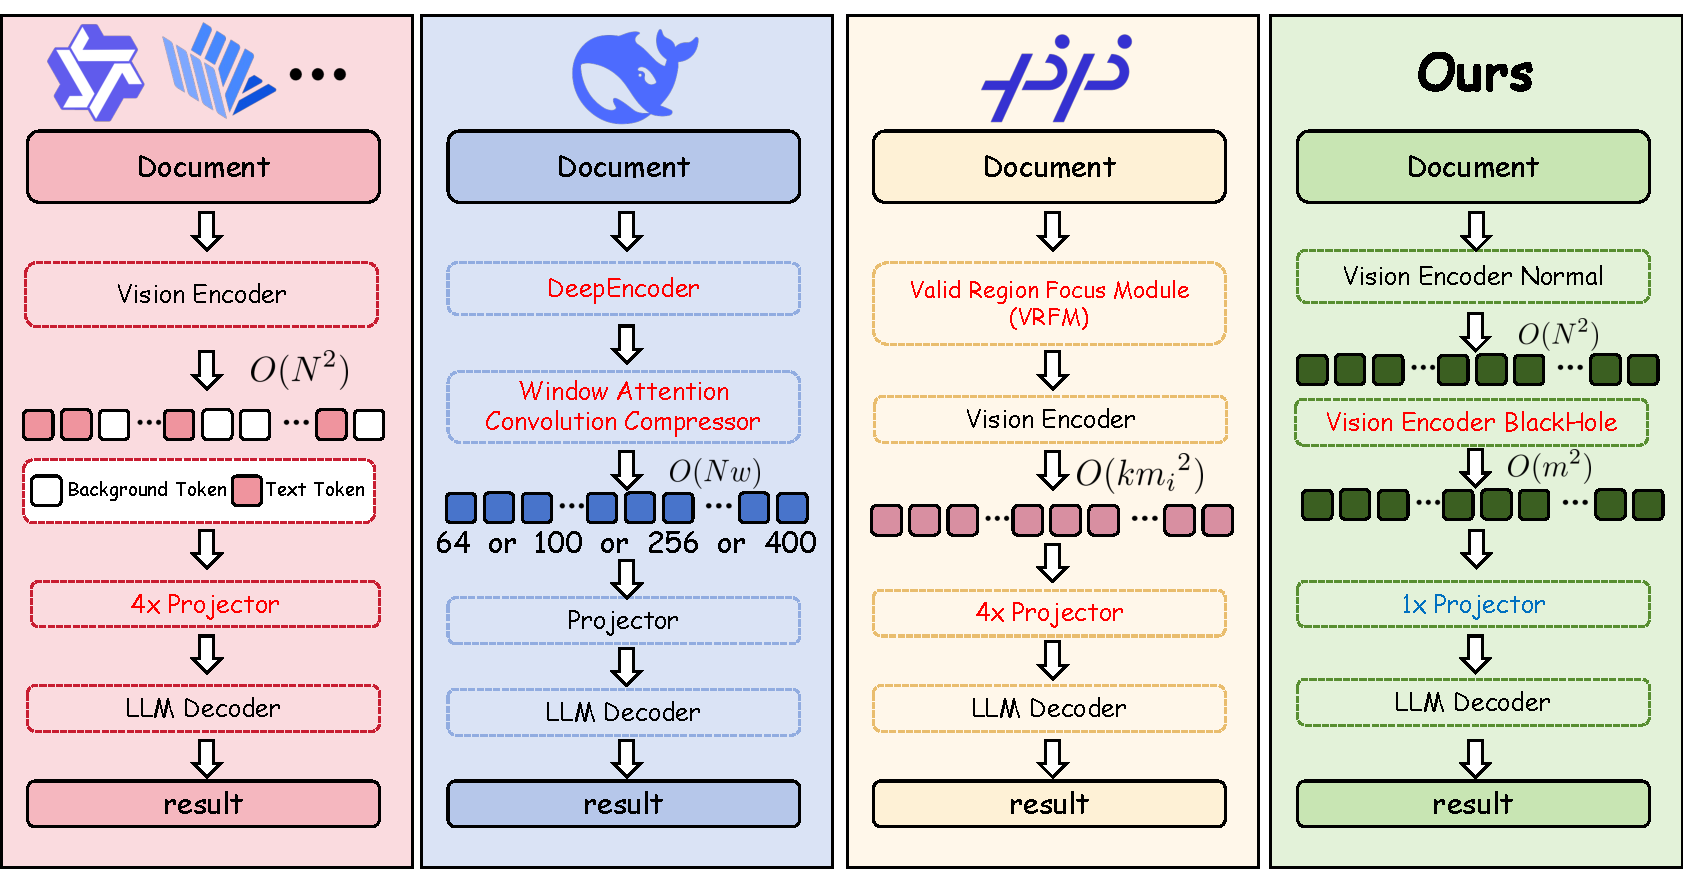
\includegraphics[width=\linewidth]{figures/final/compare_model.pdf}
\caption{Comparison between existing document parsing pipelines and \ours{}. Unlike fixed compression or external region selection, \ours{} reallocates the visual token budget inside the ViT according to document content density.}
\end{figure}

Existing compression methods do not fully resolve this mismatch. Fixed projectors or downsampling cannot distinguish text-dense regions from blank areas. Token pruning shortens the sequence, but directly removes discarded information. Token merging preserves more information than pruning, but usually relies on fixed ratios or global thresholds and therefore cannot adapt its compression strength to each page. Multi-stage OCR systems can crop redundant regions with external layout modules, but they change the setting of end-to-end VLMs and introduce additional detectors. This leads to a key question: without introducing an external detector, can an end-to-end document VLM infer from its own representations which visual tokens should be preserved first and which information can be compressed?

Our answer is yes. We find that the L2 norm of ViT Key vectors in pretrained document VLMs provides an annotation-free signal of content density. Across multiple OCR/document VLMs, text and structured content regions usually have higher K-norms, while background regions have lower K-norms. Based on this observation, we propose \ours{}, a content-adaptive visual token merging method for end-to-end document VLMs. At an intermediate ViT layer, \ours{} converts K-norms into density scores, keeps high-density tokens as local representatives, and merges low-density tokens into retained tokens according to K-vector similarity. In this way, important content is preserved first, while secondary content is compressed rather than hard-pruned, avoiding the information loss of pruning and the content-independent schedule of fixed merging.

To obtain stable compression decisions, \ours{} further uses merge-aware supervised fine-tuning to adapt the model to merged visual representations, and lightweight reinforcement learning to learn sharper keep/merge boundaries under quality constraints. We validate \ours{} on multiple end-to-end document VLM settings. Experiments show that it substantially reduces visual tokens with nearly lossless parsing accuracy, achieving over 70\% average visual token compression on OmniDocBench v1.6.